%!TEX root = proposal.tex

\section{Introduction}

The goal of this project is to explore the possibility of incorporating a machine in the loop of collaborative writing.
Collaborative writing is ubiquitous, ranging from the creation of Wikipedia by millions of online volunteers, to the draft of legislative bills by congress representatives, to routine business activities such as crafting a slogan for a marketing campaign by a small team.
Thanks to tools such as Office 365, Google Doc, and Wikimedia, collaborative writing is increasingly digitalized.
However, there is limited {\em intelligent} support in this collaborative writing process despite its prevalence \citep{gehrmann2015deploying}.

% \chenhao{The exciting level of the introduction is kind of low.}

This proposal aims to develop the best practices for providing intelligent support in collaborative writing.
We propose a general machine-in-the-loop framework to enable a team to collaborative effectively in the writing process.
% , building on our prior work on creative writing with individuals \citep{clark+etal18}.
In this case, our machine-in-the-loop systems are composed of a team of multiple people and a machine working together to create output (\figref{fig:task}). The team and machine are in a loop in which the team provides context and the machine responds with suggestions to the team. The team controls the final output.
We would like to emphasize two points in this framework:
1)  The team is the central agent. Machine learning systems in this framework are developed to assist humans in its best possible way rather than to outperform humans or achieve an absolute sense of intelligence.
2)  In order for this process to be successful, the suggestions made by the machine should be helpful, but do not need to be directly copied as final outcomes.
In other words, we emphasize increasing productivity over building intelligent AI.
% \chenhao{should emphasize collaboration a bit more if we are submitting for human collaboration.}

\begin{figure}[t]
\centering
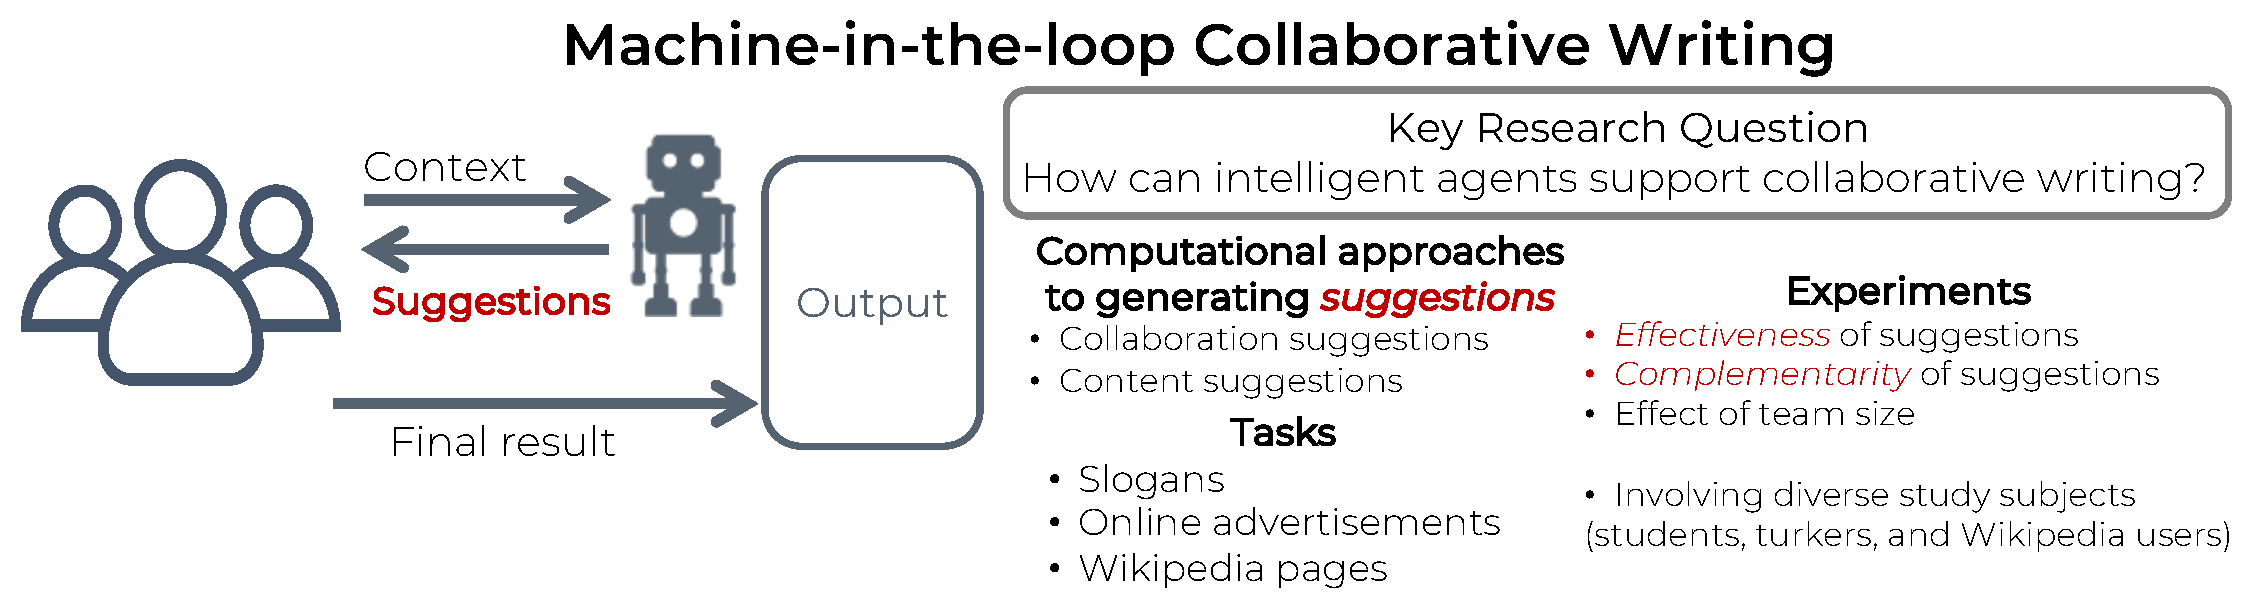
\includegraphics[width=0.85\textwidth]{illustration.pdf}
\caption{An overview of machine-in-the-loop collaboration and the proposed research.}
\label{fig:task}
\end{figure}

Specifically, we will 1) develop computational approaches to generating appropriate suggestions in the collaborative writing process and 2) design large-scale user studies to understand the role of an intelligent machine in the collaborative writing process and evaluate the effectiveness of machine-in-the-loop approaches.
% \chenhao{we should try to emphasize why this is different from clippy.}
We consider two types of suggestions:
1) collaboration suggestions that aim to improve the work-flow in the collaborative writing process by recommending topics and structures of collaboration.
Such suggestions are unique to collaborative writing, compared to individual writing.
2) content suggestions that help the human team overcome cognitive inertia.
Preliminary findings from our pilot study on slogan writing with a machine in the loop motivate us to pursue lexical suggestions instead of full-sentence suggestions in this proposal.
Lexical suggestions can help least in two ways.
First, in the early stage of writing, some words can help brainstorm ideas, e.g., relevant keywords that violate common norms but remain benign according to benign violation theory \citep{warren_opinion:_2015}.
Second, lexical suggestion can help the team identify the most appropriate word in terms of sentiment, connotation, rhyme, alliteration, etc.
It also removes the concern of grammaticality for generating full sentences.

Our experimental evaluations considers multiple writing tasks (i.e., slogans, online advertisements, and Wikipedia pages) and experimental settings to evaluate the proposed computational suggestions.
We will focus on synchronous collaboration between two people and explore the design space of pull vs. push in offering suggestions.
Our experiments will answer the following research questions:
1) {\em how collaboration suggestions shape the collaboration process};
2) {\em how content suggestions assist human teams in different stages of writing};
3) {\em how collaboration suggestions and content suggestions complement each other in collaborative process}.
In addition to pilot studies with college students and large-scale user studies with Mechanical Turkers, we will also explore realistic collaboration with Wikipedia contributors.

% \subsection{Connection to Productivity}

% \subsection{Expected Results and Broader Impacts}

\para{Expected results.} We expect to build a collaborative writing web application that can serve as a common experimentation platform for future research in machine-in-the-loop collaborative writing.
We will also contribute novel computational algorithms/models for providing collaboration and content suggestions.
Finally, our experiments will reveal insights about the collaboration between human teams and AI systems.

\para{Broader impacts.} The proposed research will promote the positive role of AI in our society.
By focusing on a ubiquitous yet understudied domain, collaborative writing, the proposed research will lay the foundation for future research in this area.
Given that one of our proposed task is to write Wikipedia pages, it also holds promise in contributing directly to a significant non-profit effort on the Internet.